\section{Portfolio Learnability}
\label{sec:portfolio_learnability}

\subsection{A Class of Portfolio Economies}
\label{sec:economy_class}

For the fixed representation in Assumption~\ref{ass:kernel}, fix $b>1$,
$\gamma>b$, constants $C_\beta,B_X,R>0$, $K_4\geq1$, and
$0<c_\mu\leq C_\mu<\infty$.
We denote by
\[
\mathcal E
=
\mathcal E(b,\gamma,C_\beta,B_X,K_4,R,c_\mu,C_\mu)
\]
the nonempty class of economies $\varepsilon$ satisfying the following
conditions, with all bounds common to the class:

\begin{enumerate}[label=\textup{(E\arabic*)},leftmargin=*,itemsep=0.4em]

\item\label{ec:dependence}
The process $\{(Z_t,R_{t+1})\}_{t\in\mathbb Z}$ is strictly stationary and
polynomially $\beta$-mixing, with
$\beta_\varepsilon(k)\leq C_\beta k^{-\gamma}$ for every $k\geq1$.

\item\label{ec:returns}
\textit{Gaussian-type managed-return tails and conditional fourth moments.}
Let
\[
K_t:=\bigl[K(Z_{i,t},Z_{j,t})\bigr]_{i,j=1}^N.
\]
Assume
\begin{equation}
\E_\varepsilon\!\left[
\left.
\exp\!\left(
\frac{N^{-2}R_{t+1}'K_tR_{t+1}}{B_X^2}
\right)
\right|\mathscr F_t
\right]\leq2
\quad\text{a.s.}
\label{eq:return_tail_condition}
\end{equation}
For every $V\in\Hh_K$, assume also
\begin{equation}
\E_\varepsilon\!\left[
\left.(R^p_{t+1}(V))^4\right|\mathscr F_t
\right]
\leq
K_4
\left\{
\E_\varepsilon\!\left[
\left.(R^p_{t+1}(V))^2\right|\mathscr F_t
\right]
\right\}^2
\quad\text{a.s.}
\label{eq:conditional_fourth_condition}
\end{equation}
Both bounds are uniform over the class. Since
$N^{-2}R_{t+1}'K_tR_{t+1}=\|X_t\|_{\Hh_K}^2$,
Condition~\eqref{eq:return_tail_condition} directly controls the diagonal
of the induced kernel while allowing unbounded returns. Conditional Gaussian
returns with uniformly bounded conditional second moments satisfy
Condition~\ref{ec:returns}; see Proposition~\ref{prop:gaussian_admissible}.

\item\label{ec:target}
The population minimum over $\Hh_K$ is attained. Its minimum-norm solution
$W^\star_\varepsilon$ satisfies $\|W^\star_\varepsilon\|_{\Hh_K}\leq R$.

\item\label{ec:pricing}
The pricing kernel $m^\star_{t+1,\varepsilon}
:=1-R^p_{t+1}(W^\star_\varepsilon)$ satisfies
\[
\E_\varepsilon\!\left[
 m^\star_{t+1,\varepsilon}R^p_{t+1}(V)
 \mid\mathscr F_t
\right]=0,
\qquad \forall\,V\in\Hh_K,
\quad\text{a.s.}
\]
Here $\mathscr F_t$ is the investor's information at the decision date in
Definition~\ref{def:economy}. Conditional pricing is imposed separately from
unconditional population optimality; positivity is not imposed.

\item\label{ec:spectrum}
Let $\Sigma_{\Hh_K,\varepsilon}=\E_\varepsilon[X_t\otimes X_t]$ and let
$\mu_{1,\varepsilon}\geq\mu_{2,\varepsilon}\geq\cdots>0$ denote its positive
eigenvalues. Then
\[
c_\mu j^{-b}\leq\mu_{j,\varepsilon}\leq C_\mu j^{-b},
\qquad j\geq1.
\]

\item\label{ec:sharpe}
The optimal payoff has positive
variance and $\SR^\star_{\varepsilon,K}:=\SR(R^p_{t+1}(W^\star_\varepsilon))$
satisfies the common bounds
\[
0<\underline S\leq\SR^\star_{\varepsilon,K}\leq\overline S<\infty.
\]
\end{enumerate}

Condition~\ref{ec:returns} replaces the almost-sure bounded-return restriction
by Gaussian-compatible tail and fourth-moment control. Proposition~\ref{prop:gaussian_admissible}
in Appendix~\ref{app:primitive_consequences} gives a simple sufficient
conditional-Gaussian specification. No Gaussianity is otherwise imposed.

The class $\mathcal E$ separates two forces governing portfolio learnability.
The exponent $\gamma$ controls the persistence of the data, while $b$ controls
the geometry of the managed-portfolio spectrum.
The parameter $b$ describes how concentrated the managed-portfolio opportunity
set is. A large $b$ means that most payoff variation is concentrated in a
relatively small number of strong portfolio directions. A smaller $b$ leaves a
longer tail of economically distinct but progressively weaker directions.

Polynomial spectral decay is natural for finite-smoothness representations,
including Sobolev--Mat\'ern, Laplace, and spline-type kernels. Gaussian kernels
can instead generate exponential or faster-than-polynomial decay
\citep{belkin2018}. For exposition, we use $b=\infty$ as shorthand for the
fast-decay benchmark, including Gaussian-type spectra and the finite-rank
limit. The class $\mathcal E$ itself has finite $b$; these are separate
benchmarks, not substitutions into the restriction $\gamma>b$.
Their relevance depends on the spectrum of $\Sigma_{\Hh_K,\varepsilon}$,
not on the kernel name alone.

\subsection{Learnable Sharpe ratio and optimal shrinkage}

We can now ask how regularization should change as market history accumulates,
how rapidly the population maximum-Sharpe direction can be recovered, and how
much of the managed-portfolio opportunity set can be reliably used. The financial observations can be 
independent over time or weakly dependent.

Population loss and Sharpe of an estimated policy hold the training sample
fixed and integrate over the stationary one-period evaluation law. They are
not the Sharpe ratio of a finite test sample.

\begin{theorem}[Optimal shrinkage and learnable frontier]
\label{thm:rate}
Choose the optimal regularization 
$$\lambda_T^\star\asymp T^{-b/(b+1)}$$, with comparison constants independent
of the economy. Uniformly over $\varepsilon\in\mathcal E$,
\begin{equation}
Q_\varepsilon(\widehat W_{\lambda_T^\star,T})
-
Q_\varepsilon(W^\star_\varepsilon)
=
O_{\mathbb P_\varepsilon}\!\left(T^{-b/(b+1)}\right).
\label{eq:portfolio-loss-rate}
\end{equation}
Moreover, uniformly over $\varepsilon\in\mathcal E$,
\begin{equation}
\SR^\star_{\varepsilon,K}
-
\SR\!\left(R^p_{t+1}(\widehat W_{\lambda_T^\star,T})\right)
=
O_{\mathbb P_\varepsilon}\!\left(T^{-b/(b+1)}\right),
\label{eq:sharpe-level-rate}
\end{equation}
where:
\[
SR_\varepsilon\!\left(\widehat W_{K,\lambda,T}\right)
=
\frac{
\mathbb E_\varepsilon
\left[
\left.
R^p_{t+1}\!\left(\widehat W_{K,\lambda,T}\right)
\right|
\widehat W_{K,\lambda,T}
\right]
}{
\sqrt{
\operatorname{Var}_\varepsilon
\left(
\left.
R^p_{t+1}\!\left(\widehat W_{K,\lambda,T}\right)
\right|
\widehat W_{K,\lambda,T}
\right)
}
}
=
\frac{
\displaystyle
\mathbb E_\varepsilon
\left[
\left.
\frac{1}{N}
\sum_{i=1}^N
\widehat W_{K,\lambda,T}(Z_{i,t})R_{i,t+1}
\right|
\widehat W_{K,\lambda,T}
\right]
}{
\displaystyle
\sqrt{
\operatorname{Var}_\varepsilon
\left(
\left.
\frac{1}{N}
\sum_{i=1}^N
\widehat W_{K,\lambda,T}(Z_{i,t})R_{i,t+1}
\right|
\widehat W_{K,\lambda,T}
\right)
}
}
\]
and
\[
SR^\star_{\varepsilon,K}
=
\sup_{W\in\mathcal H_K}
\frac{
\mathbb E_\varepsilon
\left[
\frac{1}{N}
\sum_{i=1}^N
W(Z_{i,t})R_{i,t+1}
\right]
}{
\sqrt{
\operatorname{Var}_\varepsilon
\left(
\frac{1}{N}
\sum_{i=1}^N
W(Z_{i,t})R_{i,t+1}
\right)
}
}.
\]
\end{theorem}

The theorem first establishes consistency of direct portfolio learning. Since
$\lambda_T^\star\rightarrow0$ and
$
\SR_K^\star
-
\SR\!\left(
\widehat W_{\lambda_T^\star,T}
\right)
\rightarrow_P0,
$
the portfolio manager eventually recovers the maximum-Sharpe direction
available within the chosen portfolio representation.

The optimal regularization path also gives a dynamic interpretation to the
eigenportfolio logic discussed above. With a short return history, directions
deep in the managed-portfolio spectrum are weakly identified and are therefore
shrunk heavily. As more observations become available, their expected payoff
and payoff variation can be estimated more precisely, allowing the manager to
take progressively larger positions in those directions.

Indeed, as
$
\lambda_T^\star
\asymp
T^{-b/(b+1)}
$
falls with $T$, the spectral filter
$
\frac{\mu_j}
{\mu_j+\lambda_T^\star}
$
moves toward one for progressively smaller values of $\mu_j$. Directions that
were effectively suppressed in short samples therefore become statistically
usable in longer samples.

Regularization is thus a finite-history device. More data allow the portfolio manager to move
deeper into the managed-portfolio spectrum and exploit investment opportunities
that were previously too weakly identified.

The shape of the spectrum determines how quickly portfolio opportunities can be
learned. A steep spectrum (large $b$) concentrates economically relevant payoff
variation in a few directions, making the portfolio easier to learn. A flatter
spectrum spreads variation across many weaker directions, increasing potential
breadth but slowing learning.


Importantly, portfolio learnability is therefore not determined directly by the
number $D$ of firm characteristics. Two representations with the same number of
characteristics can generate very different learning problems. If their
characteristics produce largely redundant portfolio bets, the managed-portfolio
spectrum is concentrated. If instead they produce many distinct but weak
portfolio directions, the spectrum is diffuse and substantially more market
history is required.

What matters for the portfolio manager is therefore not the raw number of
signals, but the economic geometry of the portfolios generated by those
signals.

Figure~\ref{fig:learnable_frontier} gives a graphical interpretation of the learning result: as market history grows, the learned capital-allocation line rotates toward the population tangency line. Under Condition~\ref{ec:sharpe}, at any fixed volatility, the expected-return gap closes at rate $O_P\!\left(T^{-b/(b+1)}\right)$.

\Needspace{0.82\textheight}
\begin{figure}[H]
\centering
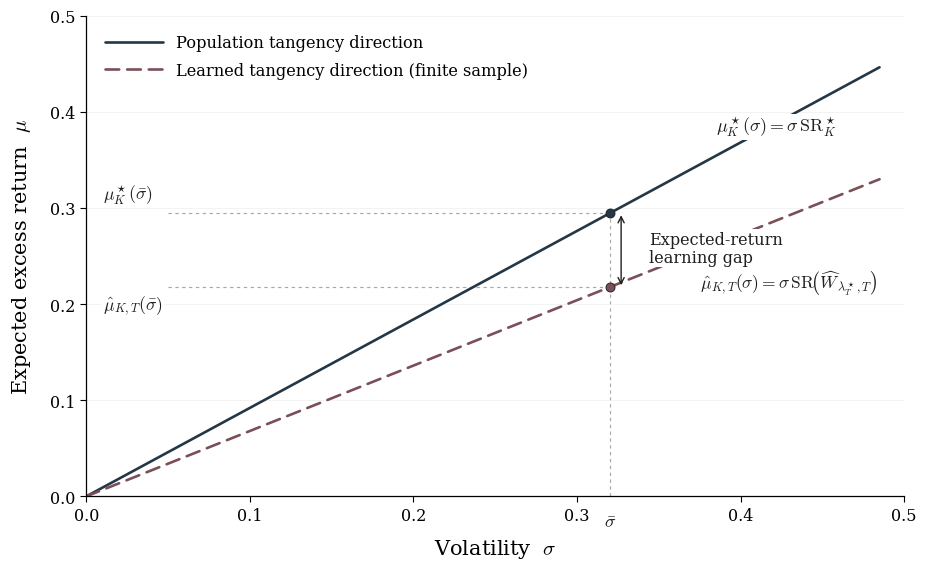
\includegraphics[width=0.93\textwidth]{figures/FRONTIER.png}
\caption{\textbf{Learning the tangency direction.}
The population tangency direction generates expected excess return
$\mu_K^\star(\sigma)=\sigma\SR_K^\star$, while the direction learned from a
finite history generates
$\hat\mu_{K,T}(\sigma)
=\sigma\SR(\widehat W_{\lambda_T^\star,T})$.
At the fixed volatility target $\bar\sigma$, the vertical distance is the
expected-return learning gap
$\mu_K^\star(\bar\sigma)
-\hat\mu_{K,T}(\bar\sigma)$.}
\label{fig:learnable_frontier}
\end{figure}




\subsection{Optimal effective portfolio complexity}



The optimal-shrinkage result can now be expressed directly in terms of
portfolio complexity.

\begin{theorem}[Learnable effective portfolio complexity]
\label{thm:effective_complexity}
Under the portfolio-loss conditions of Theorem~\ref{thm:rate}, the rate-optimal effective complexity satisfies
\begin{equation}
\mathcal C_{K,T}^\star
:=
\mathcal C_K(\lambda_T^\star)
\asymp
T^{1/(b+1)}.
\label{eq:optimal_complexity}
\end{equation}
\end{theorem}

The theorem gives a direct economic interpretation of additional market
history. As $T$ increases and optimal shrinkage declines, the portfolio manager
can reliably activate a broader set of managed-portfolio directions.

This expansion is nevertheless gradual. Effective complexity grows
sublinearly:
$
\frac{\mathcal C_{K,T}^\star}{T}
\rightarrow
0.
$
Thus, even when the underlying representation is arbitrarily rich, a finite
market history supports only a limited fraction of its potential portfolio
directions.

A steep managed-portfolio spectrum implies slower growth of effective
complexity because most economically relevant payoff variation is already
concentrated in a few strong directions. A flatter spectrum supports greater
potential breadth, but exploiting that breadth requires substantially more
market history.

Figure~\ref{fig:optimal-effective-complexity} summarizes this tradeoff. With a
short history, the Sharpe-maximizing portfolio uses only a small number of
effective directions. With more observations, weaker directions become
reliably investable and the optimal effective complexity shifts outward.

\begin{figure}[H]
\centering
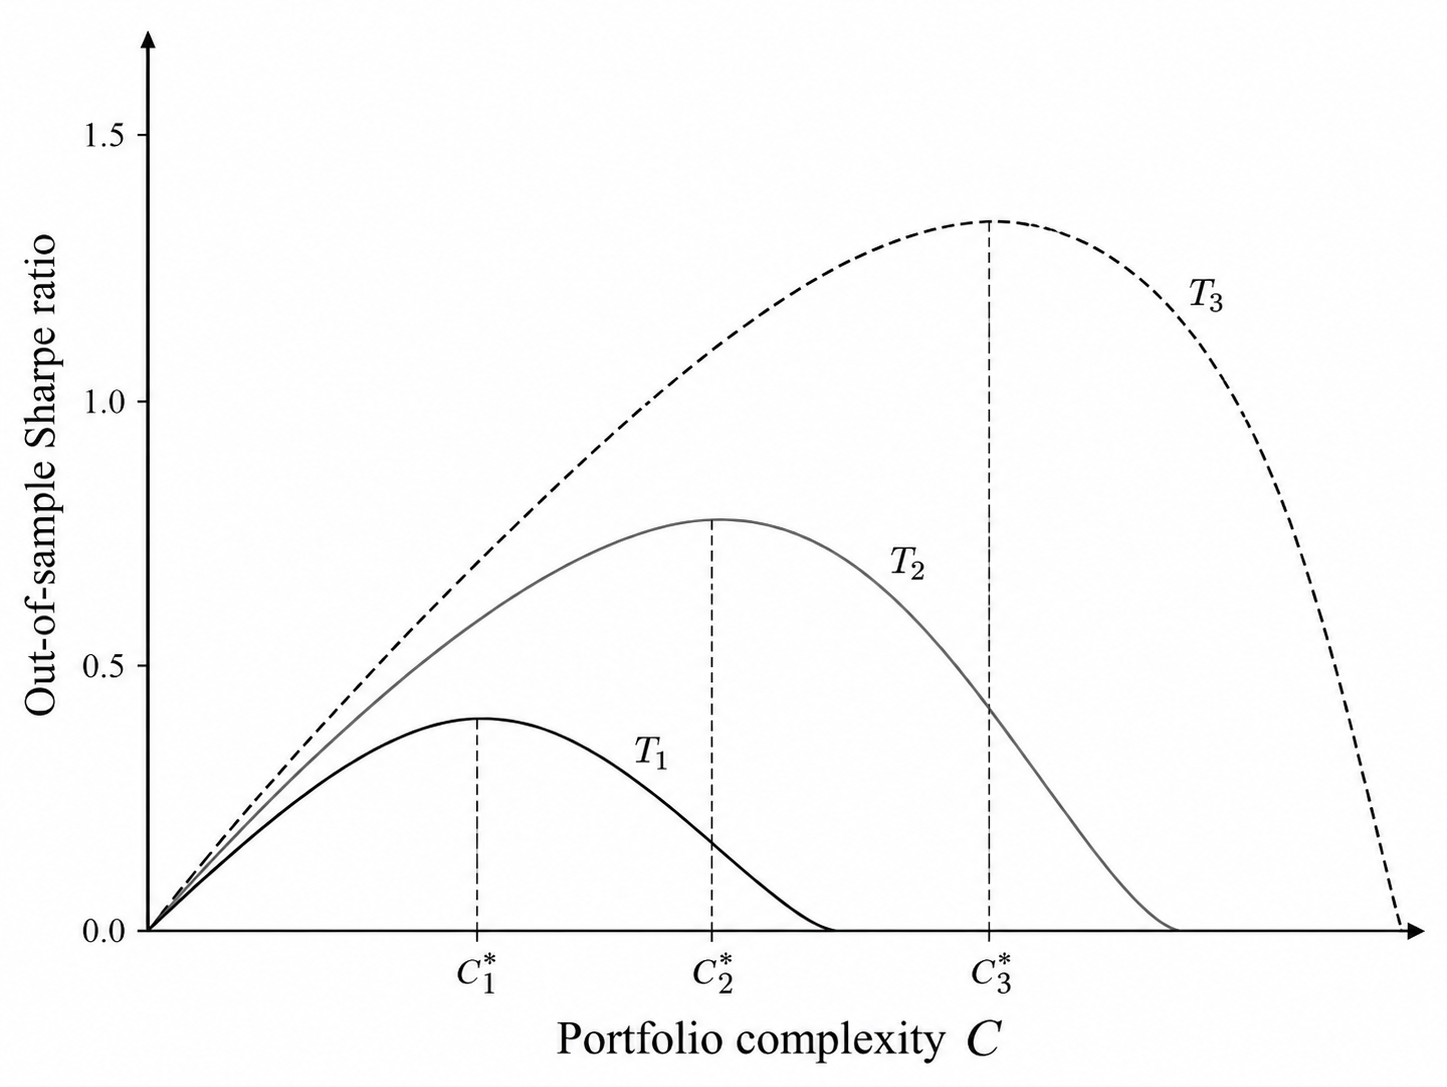
\includegraphics[width=0.94\textwidth]{figures/Complexity.png}
\caption{\textbf{Market history and learnable portfolio complexity.}
Schematic Sharpe--complexity profiles for different history lengths. Longer
market histories allow the portfolio manager to activate a broader set of
managed-portfolio directions, shifting the Sharpe-maximizing effective
complexity to the right.}
\label{fig:optimal-effective-complexity}
\end{figure}

The distinction from nominal size is central. A large representation expands
the set of portfolio policies that can potentially be expressed. Effective
complexity measures how much of that representation the portfolio manager can
actually use given the available history of returns. Effective complexity is therefore a
learnable economic that quantify the amount of eigenportoflios that the portoflio manager trade.






\subsection{The fundamental limit}
\label{sec:minimax}

The previous results describe how a portfolio manager should use a finite
market history: weak managed-portfolio directions should be shrunk, the amount
of shrinkage should decline as more observations become available, and the
set of portfolio opportunities that can be reliably exploited expands with
the sample. A natural question remains. Could a different learning technology
overcome this limitation? Could a sufficiently large neural network, a richer
random-feature model, or a more sophisticated portfolio algorithm recover the
optimal investment decision substantially faster?

The answer is no without additional economic structure.

\begin{theorem}[Fundamental limit of maximum-Sharpe learning]
\label{thm:minimax_words}
There exists a constant $c>0$ such that, for all sufficiently large $T$,
\[
\inf_{\widetilde W_T}
\sup_{\varepsilon\in\mathcal E}
\mathbb E_\varepsilon
\left[
\SR^\star_{\varepsilon,K}
-
\SR_\varepsilon
\!\left(
R^p_{t+1}(\widetilde W_T)
\right)
\right]
\ge
c\,T^{-b/(b+1)}.
\]
The infimum is over all measurable portfolio-learning procedures based on the
$T$ observed financial rows. Hence no portfolio-learning procedure can
uniformly recover the population maximum Sharpe ratio at a faster rate than
$T^{-b/(b+1)}$ over $\mathcal E$.
\end{theorem}

Together with Theorem~\ref{thm:rate}, this establishes $T^{-b/(b+1)}$ as the minimax-optimal rate for learning the maximum Sharpe ratio over the class considered here.

The limitation is therefore informational rather than computational. Portfolio
directions deep in the managed-payoff spectrum are only weakly identified by a
finite history of realized returns. A richer model may represent more
investment opportunities, and a better algorithm may use the available
information more effectively, but neither can make those weakly identified
opportunities more visible in the data.

Learning faster requires knowing more about the economy. This can come from a
longer market history or from additional economic restrictions on the return
process, the managed-payoff spectrum, or the location of optimal portfolio
demand. Absent such information, the learning rate is a property of the
investment problem, not of the particular algorithm used to solve it.